\chapter{Modeling Correlation between Risks}

In credit derivative valuation and credit risk management, one of the
fundamentally important issues is the estimate of default
probabilities and their correlations. For this, generally speaking,
there are two ways: using historical default data or using mathematical
models.

Historical default data has played an important role in the estimate
of default probabilities. However, because credit events are rare,
there is very limited default data available. Moreover, historical data only
reflects the past default pattern and it may not be a proper
indicator of the future. This makes the estimate of default
probabilities from historical data difficult and inexact. To use this
same data to estimate default correlations is even more difficult and
inexact.

The market trend now is towards the use of mathematical
models that don't rely on historical default data. In
Chapter~\ref{credit_default_swaps} we have seen how it is possible to derive default probabilities from market data,
here we will see how the copula can be used to model their correlations. 

\section{One Factor Gaussian Copula Model}
\label{standard-market-model}
While there are several types of copula function models, the first
introduced was the \emph{one-factor Gaussian copula model}. This model 
is quite simple and has, above all, the advantage that can be solved semi-analytically.
In essence the one-factor Gaussian copula, is nothing but a numerical algorithm to generate samples of normally distributed random variables that have a given
pair-wise correlation. 

Consider a portfolio of \(N\) bonds and assume that the marginal
probabilities of default are known for each issuer. Define:

\begin{itemize}
	\tightlist
	\item
	\(t_i\), the time of default of the \(i^{th}\) company:
	\item
	\(Q_i(t)\), the cumulative probability that company \(i\) will default
	before time \(t\); that is, the probability that \(t_i \le t\).
\end{itemize}

To generate a one-factor model for the default times (\(t_i\)) we define random
variables \(X_i\) \((1\le i \le N)\)
\begin{equation}
X_i = a_i M + \sqrt{1-a_i^2}Z_i,\qquad i = 1, 2,\ldots, N
\label{eq:normalized_var}
\end{equation}
where \(M\) and the \(Z_i\) are independent zero-mean unit-variance  distributions (hence $X_i$ are also distributed with zero-mean and unit standard-deviation) and \(-1 \le a_i \lt 1\).

Eq.~\ref{eq:normalized_var} defines a correlation structure between the
\(X_i\) which are dependent on a single common factor \(M\). The $Z_i$ term is usually called the idiosyncratic component of default. 
The particular functional form of Eq.~\ref{eq:normalized_var} has been chosen 
to ensure the desired correlation structure among the $X_i$.
Indeed the correlation between \(X_i\) and \(X_j\) is

\begin{equation*}
\rho(X_i, X_j) = \cfrac{\mathbb{E}[(X_i-\mu_i)(X_j-\mu_j)]}{\sigma_{i}\sigma_{j}} =\mathbb{E}[X_i X_j] = a_i a_j \mathbb{E}[M^2] = a_i a_j
\end{equation*}
where we just exploit the definition of $X_i$ and its properties.

%Assume that the $i^{th}$ company has defaulted by the time $t_i$ if $X_i$ is below a threshold value $\bar{x}_i(t_i)$.
If $F_i$ is the cumulative distribution function of the $X_i$,
with a percentile to percentile transformation (see Section~\ref{distribution-transformation}) we can map the \(X_i\) to the \(t_i\), so that $Q_i(t_i) = P(X_i\le x)=F_i(x)$.
Therefore a point \(X_i = x\) is transformed to \(t_i = t\) with
\(x = F_i^{-1}[Q_i(t)]\).

Let's note that, \textbf{conditional} on $M$, the $N$ default events are \textbf{independent}. So we can write
\begin{equation}
\begin{split}
Q_i^{\textrm{corr}}(t_i|M) = P(X_i\le x|M) &= P(a_i M + \sqrt{1-a_i^2}Z_i\le x) =\\
&= P\left(Z_i\le \cfrac{x-a_i M}{\sqrt{1-a_i^2}}\right)
=H_i\left(\cfrac{F^{-1}[Q(t_i)]-a_i M}{\sqrt{1-a_i^2}}\right)
\end{split}
\label{eq:generic_copula}
\end{equation}
where $H_i$ is the cumulative distribution function of the $Z_i$.

Although in principle any distribution could be used for \(M\) and the
\(Z\)'s (provided they have zero mean and unit variance), one common
choice is to let them be standard normal distributions (resulting in a
Gaussian copula).
So we can rewrite Eq.~\ref{eq:generic_copula} as

\begin{equation}
Q_i^{\textrm{corr}}(t_i|M) = \Phi\left(\cfrac{\Phi^{-1}[Q(t_i)]-a_i M}{\sqrt{1-a_i^2}}\right)
\label{eq:gaussian_one_factor_copula}
\end{equation}
where $\Phi$ denotes the cumulative distribution function of the standard normal distribution.

If we call $\mathcal{C}(t_1,\ldots,t_N)$ the joint distribution of the default times of the $N$ bonds in the portfolio then

\begin{equation}
\mathcal{C}(t_1,\ldots,t_N, \rho)=\Phi(\Phi^{-1}(Q_1(t_1)),\ldots,\Phi^{-1}(Q_N(t_N)), \rho)
\end{equation}
where $\rho$ represents the correlation matrix of the default probabilities, is the one factor Gaussian copula model (one factor because there is only a random variable, $M$, which determines the correlation between $X_i$).

Clearly different choices of distributions result in different copula models, and in various natures of the default dependence. For example, copulas where the \(M\) have heavy tails generate models where there is a
greater likelihood of a clustering of early defaults for several
companies.

\subsection{Standard Market Model}\label{standard-market-model}

Assume the following two assumptions are made:

\begin{itemize}
	\tightlist
	\item
	all the companies have the same default intensity (hazard rates), i.e, \(\lambda_i = \lambda\) (which means they all have the same default probabilities $Q_i = Q$);
	\item
	the pairwise default correlations are the same, i.e \(a_i = a\); in other words the contribution of the market
	component $M$ is the same for all the companies and the correlation between any two companies is constant, \(\rho = a^2\).
\end{itemize}

Under these assumptions, given the market situation \(M = m\), all the
companies have the same cumulative default probability
\(Q_i^{\textrm{corr}}(t_i|m)=P(X_i < x|m)\). 
Moreover, for a given value of the
market component \(M\), the defaults are mutually independent for all
the underlying companies. 

With the assumption that have been made the one factor model is also called \emph{Market Standard Model}.
Later in this Chapter we will also see how the correlation used in Eq.~\ref{eq:gaussian_one_factor_copula} can be implied from the market quotes of 
credit derivatives.

Letting \(l(t|m)\) be the total defaults that
have occurred by time \(t\) conditional on the market condition
\(M = m\), then \(l(t|m)\) follows a binomial distribution (see Appendix~\ref{binomial-distribution}), and the default probability $DP$ of $j$ companies
can be expressed as

\begin{equation}
DP(l(t|m) = j) = \cfrac{N!}{j!(N-j)!}(Q_i^{\textrm{corr}}(t_i|m))^j(1-Q_i^{\textrm{corr}}(t_i|m))^{N-j},\qquad  j=0, 1, 2,\ldots,N
\end{equation}

In general to evaluate any function $g(DP(l(t))$ regardless the parameter $M$
(e.g. an NPV or a fair value which depend on the default probability, remember~\ref{sec:cds_valuation}) is necessary to average according to all the possible values that $M$ can take. The average is performed with an integral which is the weighted sum of $g$ with the probability distribution ($f_M(m)$) of the random variable $M$  

\begin{equation}
g(DP(l(t) = j)) = \int_{-\infty}^{\infty}{g(DP(l(t|m) = j))\cdot f_M(m)dm}
\label{eq:gaussian_quadrature}
\end{equation}

In the general case where the default probabilities of each company are not the same 
it is possible to determine $DP(l(t|M)=j)$ through an iterative procedure before
proceeding with the integration of Eq.~\ref{eq:gaussian_quadrature}.
An example of this iterative technique will be shown in Section~\ref{sec:expected_losses}.

\subsection{Extensions of the One Factor Copula Model}
Many other one-factor model have been tried: t-Student copula, Clayton copula, \ldots In general we can define a new model by simply choosing particular functional forms for $M$ and $Z_i$ in Eq.~\ref{eq:normalized_var} provided they are with zero mean and standard deviation one. 

If instead of the single factor $M$ there are two or more, Eq.~\ref{eq:normalized_var} would become

\begin{equation}
X_i = a_1 M_1 + a_2 M_2 + \sqrt{1 - a_1^2 - a^2_2}Z_i
\end{equation}
and similarly
\begin{equation}
Q^{\textrm{corr}}(t|M_1, M_2) = \Phi\left(\cfrac{\Phi^{-1}[Q(t)]-a_1 M_1 - a_2 M_2}{\sqrt{1 - a_1^2 - a^2_2}}\right)
\end{equation}
In terms of computation time, this kind of models are proportionally slower with the increase of the number of factors, since the integration of Eq.~\ref{eq:gaussian_quadrature} has to be carried on each random variable of the model.

\section{Basket Default Swaps}\label{basket-default-swaps}

A Basket Default Swap is a credit derivative on a portfolio of reference
entities. The simplest basket default swaps are first-to-default,
second-to-default, \ldots, nth-to-default swaps. 

This kind of contracts are very similar to normal CDS except for the protection they offer.
With respect to a basket of reference entities, a first-to-default swap provides insurance for only the first default, a second-to-default swap provides insurance
for only the second default, or a nth-to-default swap provides insurance for only the $n^{th}$ default. 

For example, in the last case, the seller does not make a payment to the protection buyer for
the first $n-1$ defaulted reference entities, and makes a payment only for the
$n^{th}$ defaulted reference entity. Once there has been this payment the swap terminates.

The cost of protection in nth-to-default basket is obviously dependent on default correlations. 
Suppose that a basket of 100 reference entities is used to define a 5-year nth-to-default CDS and that each reference entity has a 2\% probability of defaulting during the next
5 years. When the default correlation between the reference entities is zero, the binomial distribution (see Appendix~\ref{binomial-distribution}) 
shows that the probability of one or more defaults during 5 years is 86.74\% and the probability of ten or more defaults is 0.0034\%.

\begin{codebox}
\begin{Verbatim}[commandchars=\\\{\}]
\PY{k+kn}{from} \PY{n+nn}{scipy}\PY{n+nn}{.}\PY{n+nn}{stats} \PY{k}{import} \PY{n}{binom}
	
\PY{n}{b} \PY{o}{=} \PY{n}{binom}\PY{p}{(}\PY{l+m+mi}{100}\PY{p}{,} \PY{l+m+mf}{0.02}\PY{p}{)}
\PY{n+nb}{print}\PY{p}{(}\PY{l+s+s2}{\PYZdq{}}\PY{l+s+s2}{P(\PYZgt{}=1) : }\PY{l+s+si}{\PYZob{}\PYZcb{}}\PY{l+s+s2}{\PYZdq{}}\PY{o}{.}\PY{n}{format}\PY{p}{(}\PY{l+m+mi}{1} \PY{o}{\PYZhy{}} \PY{n}{b}\PY{o}{.}\PY{n}{cdf}\PY{p}{(}\PY{l+m+mi}{0}\PY{p}{)}\PY{p}{)}\PY{p}{)}
\PY{n+nb}{print}\PY{p}{(}\PY{l+s+s2}{\PYZdq{}}\PY{l+s+s2}{P(\PYZgt{}=10): }\PY{l+s+si}{\PYZob{}\PYZcb{}}\PY{l+s+s2}{\PYZdq{}}\PY{o}{.}\PY{n}{format}\PY{p}{(}\PY{l+m+mi}{1} \PY{o}{\PYZhy{}} \PY{n}{b}\PY{o}{.}\PY{n}{cdf}\PY{p}{(}\PY{l+m+mi}{9}\PY{p}{)}\PY{p}{)}\PY{p}{)}
	
P(>=1) : 0.8673804441052471
P(>=10): 3.441680604299169e-05
\end{Verbatim}
\end{codebox}

A first-to-default is therefore quite valuable whereas a tenth-to-default CDS is worth almost nothing.

As the default correlation increases the probability of one or more defaults declines 
but that for ten or more defaults increases. In the limit where default correlations are perfect the probability of one or more defaults equals the probability of ten or more and it is 2\%. This is because in this extreme situation the reference entities are essentially the same: either they all default (with 2\% probability) or none of them default (with 98\% probability).

\subsection{Basket CDS Valuation under Gaussian Copula Model}
\label{basket-cds-valuation-under-market-standard-model}
We now present some numerical results for an nth-to-default basket.
We assume that principals and expected recovery rates are the same
for all underlying reference assets. The valuation procedure is similar
to that for a regular CDS where there is only one reference entity.

In a regular CDS indeed the valuation is based on the probability that a
default occurred between times \(t_1\) and \(t_2\), see Section~\ref{sec:cds_valuation}. Here instead the valuation will be based on the probability that the $n^{th}$ default happened between times \(t_1\) and \(t_2\):
the buyer of protection makes quarterly payments at a
specified rate until the $n^{th}$ default occurs or the end life
of the contract is reached,
in case of the $n^{th}$ default occurring, the seller pays
\(F\cdot(1-R)\). 

In the following we are going to develop a \texttt{BasketDefaultSwap} class that is able to compute the basket NPV and its break-even spread.
The idea is:
\begin{itemize}
\item compute the correlated default probability of each name according to 
\begin{equation}
Q^{\textrm{corr}}(t|M) = \Phi\left(\cfrac{\Phi^{-1}[Q(t)]-\sqrt{\rho} M}{\sqrt{1-\rho}}\right)
\end{equation}
\item compute the probability of having at least $j$ defaults using the binomial distribution
\begin{equation}
DP(l(t|m) \ge j) = \sum_{k=j}^{N}\left[  \cfrac{N!}{k!(N-k)!}Q^{\textrm{corr}}(t|M)^k(1-Q^{\textrm{corr}}(t|M))^{N-k}\right]
\end{equation}
\item create a \textbf{credit curve}, $CC(DP)$ with those probabilities;
\item re-use the \texttt{CreditDefaultSwap} class methods to compute NPV and break-even rate (with the appropriate discount curve and the credit curve determine above), through integration of
\begin{equation}
\mathrm{NPV}(DC, CC(DP)) = \int_{-\infty}^{\infty}{\mathrm{NPV}(DC, CC(DP)) f_M(m)dm} 
\end{equation}
and similarly for the break-even rate.
\end{itemize}

Since to valuate a basket default swap we need to perform integrals let's see briefly how it works in \texttt{python}.

To integrate a function \(f\) we can use \(\tt{scipy.integrate.quad}\) which takes in
input: the function to integrate, the integration limits and, if needed, optional arguments of the integrand (see Section~\ref{sec:kwargs_args}). Since it is a numerical integration the result will be a tuple with the actual value and the associated error (we will always be interested in the first item only though).

For example imagine to integrate
\[f(x) = \int_{-2}^{4}(ax^{3} + b)~dx\]
for \(a=3\) and \(b=5\)

\begin{codebox}
\begin{Verbatim}[commandchars=\\\{\}]
\PY{k+kn}{from} \PY{n+nn}{scipy}\PY{n+nn}{.}\PY{n+nn}{integrate} \PY{k}{import} \PY{n}{quad}
	
\PY{k}{def} \PY{n+nf}{func}\PY{p}{(}\PY{n}{x}\PY{p}{,} \PY{n}{a}\PY{p}{,} \PY{n}{b}\PY{p}{)}\PY{p}{:}
    \PY{k}{return} \PY{n}{a}\PY{o}{*}\PY{n}{x}\PY{o}{*}\PY{o}{*}\PY{l+m+mi}{3} \PY{o}{+} \PY{n}{b}
	
\PY{n}{s} \PY{o}{=} \PY{n}{quad}\PY{p}{(}\PY{n}{func}\PY{p}{,} \PY{o}{\PYZhy{}}\PY{l+m+mi}{2}\PY{p}{,} \PY{l+m+mi}{4}\PY{p}{,} \PY{n}{args}\PY{o}{=}\PY{p}{(}\PY{l+m+mi}{3}\PY{p}{,} \PY{l+m+mi}{5}\PY{p}{)}\PY{p}{)}
\PY{n+nb}{print} \PY{p}{(}\PY{n}{s}\PY{p}{)}

(210.0, 2.475694446663456e-12)
\end{Verbatim}
\end{codebox}

Back to the implementation of \texttt{BasketDefaultSwaps}

\begin{codebox}
\begin{Verbatim}[commandchars=\\\{\}]
\PY{k+kn}{from} \PY{n+nn}{finmarkets} \PY{k}{import} \PY{n}{CreditCurve}\PY{p}{,} \PY{n}{CreditDefaultSwap}
\PY{k+kn}{from} \PY{n+nn}{scipy}\PY{n+nn}{.}\PY{n+nn}{stats} \PY{k}{import} \PY{n}{norm}\PY{p}{,} \PY{n}{binom}
\PY{k+kn}{from} \PY{n+nn}{numpy} \PY{k}{import} \PY{n}{sqrt}\PY{p}{,} \PY{n}{exp}, inf
\PY{k+kn}{from} \PY{n+nn}{scipy}\PY{n+nn}{.}\PY{n+nn}{integrate} \PY{k}{import} \PY{n}{quad}
		
\PY{k}{class} \PY{n+nc}{BasketDefaultSwaps}\PY{p}{:}
    \PY{k}{def} \PY{n+nf}{\PYZus{}\PYZus{}init\PYZus{}\PYZus{}}\PY{p}{(}\PY{n+nb+bp}{self}\PY{p}{,} \PY{n}{notional}\PY{p}{,} \PY{n}{names}\PY{p}{,}  \PY{n}{rho}\PY{p}{,} \PY{n}{start\PYZus{}date}\PY{p}{,} \PY{n}{spread}\PY{p}{,} 
                 \PY{n}{maturity}\PY{p}{,} \PY{n}{tenor=3}\PY{p}{,} \PY{n}{recovery=0.4}\PY{p}{)}\PY{p}{:}
        \PY{n+nb+bp}{self}\PY{o}{.}\PY{n}{names} \PY{o}{=} \PY{n}{names}
        \PY{n+nb+bp}{self}\PY{o}{.}\PY{n}{rho} \PY{o}{=} \PY{n}{rho}
        \PY{n+nb+bp}{self}\PY{o}{.}\PY{n}{cds} \PY{o}{=} \PY{n}{CreditDefaultSwap}\PY{p}{(}\PY{n}{notional}\PY{p}{,} \PY{n}{start\PYZus{}date}\PY{p}{,} \PY{n}{spread}\PY{p}{,} 
                                     \PY{n}{maturity}\PY{p}{,} \PY{n}{tenor}\PY{p}{,} \PY{n}{recovery}\PY{p}{)} 
		
    \PY{k}{def} \PY{n+nf}{one\PYZus{}factor\PYZus{}model}\PY{p}{(}\PY{n+nb+bp}{self}\PY{p}{,} \PY{n}{M}\PY{p}{,} \PY{n}{f}\PY{p}{,} \PY{n}{Q_dates}\PY{p}{,} \PY{n}{Q}\PY{p}{,} \PY{n}{dc}\PY{p}{,} \PY{n}{j}\PY{p}{)}\PY{p}{:}
        \PY{n}{DP} \PY{o}{=} \PY{n}{norm}\PY{o}{.}\PY{n}{cdf}\PY{p}{(}\PY{p}{(}\PY{n}{norm}\PY{o}{.}\PY{n}{ppf}\PY{p}{(}\PY{n}{Q}\PY{p}{)} \PY{o}{\PYZhy{}} \PY{n}{sqrt}\PY{p}{(}\PY{n+nb+bp}{self}\PY{o}{.}\PY{n}{rho}\PY{p}{)}\PY{o}{*}\PY{n}{M}\PY{p}{)}\PY{o}{/}\PY{p}{(}\PY{n}{sqrt}\PY{p}{(}\PY{l+m+mi}{1}\PY{o}{\PYZhy{}}\PY{n+nb+bp}{self}\PY{o}{.}\PY{n}{rho}\PY{p}{)}\PY{p}{)}\PY{p}{)}
        \PY{n}{b} \PY{o}{=} \PY{n}{binom}\PY{p}{(}\PY{n+nb+bp}{self}\PY{o}{.}\PY{n}{names}\PY{p}{,} \PY{n}{DP}\PY{p}{)}
        \PY{n}{S} \PY{o}{=} \PY{l+m+mi}{1}\PY{o}{\PYZhy{}}\PY{p}{(}\PY{l+m+mi}{1}\PY{o}{\PYZhy{}}\PY{n}{b}\PY{o}{.}\PY{n}{cdf}\PY{p}{(}\PY{n}{j}\PY{o}{\PYZhy{}}\PY{l+m+mi}{1}\PY{p}{)}\PY{p}{)}
        \PY{n}{cc} \PY{o}{=} \PY{n}{CreditCurve}\PY{p}{(}\PY{n}{Q_dates}\PY{p}{,} \PY{n}{S}\PY{p}{)}
        \PY{k}{return} \PY{n}{f}\PY{p}{(}\PY{n}{dc}\PY{p}{,} \PY{n}{cc}\PY{p}{)}\PY{o}{*}\PY{n}{norm}\PY{o}{.}\PY{n}{pdf}\PY{p}{(}\PY{n}{M}\PY{p}{)}
		
    \PY{k}{def} \PY{n+nf}{breakeven}\PY{p}{(}\PY{n+nb+bp}{self}\PY{p}{,} \PY{n}{Q_dates}\PY{p}{,} \PY{n}{Q}\PY{p}{,} \PY{n}{dc}\PY{p}{,} \PY{n}{ndefaults}\PY{p}{)}\PY{p}{:}
        \PY{n}{s} \PY{o}{=} \PY{n}{quad}\PY{p}{(}\PY{n+nb+bp}{self}\PY{o}{.}\PY{n}{one\PYZus{}factor\PYZus{}model}\PY{p}{,} \PY{o}{\PYZhy{}}\PY{n}{inf}\PY{p}{,} \PY{n}{inf}\PY{p}{,} 
                 \PY{n}{args}\PY{o}{=}\PY{p}{(}\PY{n+nb+bp}{self}\PY{o}{.}\PY{n}{cds}\PY{o}{.}\PY{n}{breakevenRate}\PY{p}{,} \PY{n}{Q_dates}\PY{p}{,} \PY{n}{Q}\PY{p}{,} \PY{n}{dc}\PY{p}{,} \PY{n}{ndefaults}\PY{p}{)}\PY{p}{)}
        \PY{k}{return} \PY{n}{s}\PY{p}{[}\PY{l+m+mi}{0}\PY{p}{]}
		
    \PY{k}{def} \PY{n+nf}{npv}\PY{p}{(}\PY{n+nb+bp}{self}\PY{p}{,} \PY{n}{Q_dates}\PY{p}{,} \PY{n}{Q}\PY{p}{,} \PY{n}{dc}\PY{p}{,} \PY{n}{ndefaults}\PY{p}{)}\PY{p}{:}
        \PY{n}{s} \PY{o}{=} \PY{n}{quad}\PY{p}{(}\PY{n+nb+bp}{self}\PY{o}{.}\PY{n}{one\PYZus{}factor\PYZus{}model}\PY{p}{,} \PY{o}{\PYZhy{}}\PY{n}{inf}\PY{p}{,} \PY{n}{inf}\PY{p}{,} 
                 \PY{n}{args}\PY{o}{=}\PY{p}{(}\PY{n+nb+bp}{self}\PY{o}{.}\PY{n}{cds}\PY{o}{.}\PY{n}{npv}\PY{p}{,} \PY{n}{Q_dates}\PY{p}{,} \PY{n}{Q}\PY{p}{,} \PY{n}{dc}\PY{p}{,} \PY{n}{ndefaults}\PY{p}{)}\PY{p}{)}
        \PY{k}{return} \PY{n}{s}\PY{p}{[}\PY{l+m+mi}{0}\PY{p}{]}        
\end{Verbatim}
\end{codebox}

Consider a 5-year 1st-to-default basket of ten
reference entities in the situation where copula correlation is 0.3
and the expected recovery rate, \(R\), is \(40\%\). The term structure
of interest rates is assumed to be flat at 5\%. The default
probabilities for the ten entities are generated by Poisson processes
with constant default intensities (hazard rates), \(\lambda_i=0.01\), so that

\[ Q(t) = 1 - e^{-\lambda t} \]

Using the \texttt{BasketDefaultSwap} class determine the breakeven spread.

\begin{codebox}
\begin{Verbatim}[commandchars=\\\{\}]
\PY{k+kn}{from} \PY{n+nn}{finmarkets\PYZus{}tot} \PY{k}{import} \PY{n}{DiscountCurve}
\PY{k+kn}{from} \PY{n+nn}{datetime} \PY{k}{import} \PY{n}{date}
\PY{k+kn}{from} \PY{n+nn}{dateutil}\PY{n+nn}{.}\PY{n+nn}{relativedelta} \PY{k}{import} \PY{n}{relativedelta}
\PY{k+kn}{import} \PY{n+nn}{numpy} \PY{k}{as} \PY{n+nn}{np}
	
\PY{n}{n\PYZus{}cds} \PY{o}{=} \PY{l+m+mi}{10}
\PY{n}{rho} \PY{o}{=} \PY{l+m+mf}{0.3}
\PY{n}{l} \PY{o}{=} \PY{l+m+mf}{0.01}
\PY{n}{observation\PYZus{}date} \PY{o}{=} \PY{n}{date}\PY{o}{.}\PY{n}{today}\PY{p}{(}\PY{p}{)}
	
\PY{n}{pillar\PYZus{}dates} \PY{o}{=} \PY{p}{[}\PY{n}{observation\PYZus{}date} \PY{o}{+} \PY{n}{relativedelta}\PY{p}{(}\PY{n}{years}\PY{o}{=}\PY{n}{i}\PY{p}{)} \PY{k}{for} \PY{n}{i} \PY{o+ow}{in} \PY{n+nb}{range}\PY{p}{(}\PY{l+m+mi}{6}\PY{p}{)}\PY{p}{]}
\PY{n}{dfs} \PY{o}{=} \PY{p}{[}\PY{l+m+mi}{1}\PY{o}{/}\PY{p}{(}\PY{l+m+mi}{1}\PY{o}{+}\PY{l+m+mf}{0.05}\PY{p}{)}\PY{o}{*}\PY{o}{*}\PY{n}{i} \PY{k}{for} \PY{n}{i} \PY{o+ow}{in} \PY{n+nb}{range}\PY{p}{(}\PY{l+m+mi}{6}\PY{p}{)}\PY{p}{]}
\PY{n}{dc} \PY{o}{=} \PY{n}{DiscountCurve}\PY{p}{(}\PY{n}{observation\PYZus{}date}\PY{p}{,} \PY{n}{pillar\PYZus{}dates}\PY{p}{,} \PY{n}{dfs}\PY{p}{)}
\PY{n}{Q} \PY{o}{=} \PY{p}{[}\PY{l+m+mi}{1}\PY{o}{\PYZhy{}}\PY{n}{np}\PY{o}{.}\PY{n}{exp}\PY{p}{(}\PY{o}{\PYZhy{}}\PY{p}{(}\PY{n}{l}\PY{o}{*}\PY{n}{t}\PY{p}{)}\PY{p}{)} \PY{k}{for} \PY{n}{t} \PY{o+ow}{in} \PY{n+nb}{range}\PY{p}{(}\PY{l+m+mi}{6}\PY{p}{)}\PY{p}{]}
	
\PY{n}{ndefaults} \PY{o}{=} \PY{l+m+mi}{3}
\PY{n}{basket} \PY{o}{=} \PY{n}{BasketDefaultSwaps}\PY{p}{(}\PY{l+m+mi}{1}\PY{p}{,} \PY{n}{n\PYZus{}cds}\PY{p}{,} \PY{n}{rho}\PY{p}{,} \PY{n}{observation\PYZus{}date}\PY{p}{,} \PY{l+m+mf}{0.01}\PY{p}{,} \PY{l+m+mi}{5}\PY{p}{)}
\PY{n+nb}{print}\PY{p}{(}\PY{n}{basket}\PY{o}{.}\PY{n}{breakeven\PYZus{}rate}\PY{p}{(}\PY{n}{pillar\PYZus{}dates}\PY{p}{,} \PY{n}{Q}\PY{p}{,} \PY{n}{dc}\PY{p}{,} \PY{n}{ndefaults}\PY{p}{)}\PY{p}{)}

0.0017750563139599736
\end{Verbatim}
\end{codebox}


\section{Collateralized Debt Obligation}\label{collateralized-debt-obligation}

A Collateralized Debt Obligation (CDO) is a credit derivative where the issuer 
gather risky assets and repackage them into discrete classes, called \emph{tranches}, which are defined on the level of credit risk assumed by the investor. 
These tranches of securities become the final investment product.

Tranches are named to reflect their risk profile: \emph{senior}, \emph{mezzanine} and \emph{subordinated/equity} and are delimited by an attachment ($L$) and a detachment point ($U$), which represent the percentages of the \textbf{total} principal defining their boundaries. 
For example, a 5-10\% tranche has an attachment point of 5\% and a detachment point of 10\%. 

Each of these tranches has a different level of seniority relative to the others in the sense that a senior tranche has coupon and principal payment priority over a mezzanine, while a mezzanine tranche has coupon and principal payment priority over an equity one. 

Indeed they receive returns using a set of rules known as \emph{waterfall}. Incomes of the portfolio are first used to provide returns to the most senior tranche, then to the next and so on. So senior tranches are generally safest because they have the first claim on the collateral, although they'll offer lower coupon rates.

It is important to note that a CDO only redistributes the total risk associated with the underlying pool of assets to the priority ordered tranches. It neither reduces nor increases the total risk associated with the pool.

There are various kind of CDOs:
\begin{itemize}
	\item in a \textbf{Cash CDO} the reference portfolio consists of corporate bonds owned by the CDO issuer. Cash flows from collateral are used to pay principal and interests to investors. If such cash flows prove inadequate, rewards are paid to tranches according to their seniority. Figure~\ref{fig:cdo_structure} shows a typical structure of a Cash CDO;

\begin{figure}[htb]
	\centering
	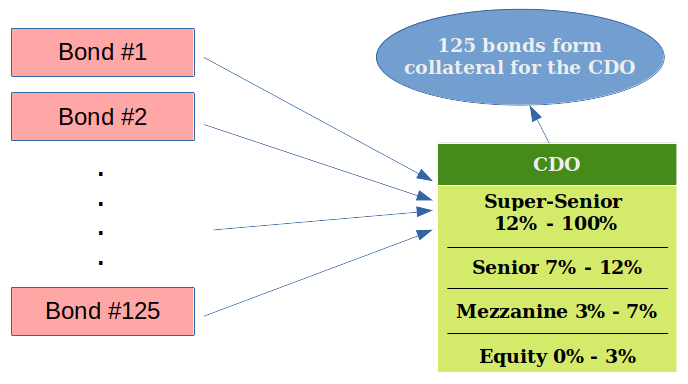
\includegraphics[width=0.7\textwidth]{figures/cdo_structure}
	\caption{Typical structure of a Cash CDO, with the reference portfolio made of bonds,
		which form the contract collateral.}
	\label{fig:cdo_structure}
\end{figure}

	\item in a \textbf{Synthetic CDO} the underlying reference portfolio is no longer "physical" (e.g. portfolio of bonds or loans), instead it is a \emph{fictitious} portfolio consisting of a number of reference obligations each with an associated notional amount. The value of a synthetic CDO usually comes from insurance premiums of credit default swaps paid for by investors. The investment logic is that sellers assume the underlying assets will perform while investors that will sooner or later default.
\end{itemize}

\subsection{Cash CDO Expected Losses}
\label{sec:expected_losses}

Consider a Cash CDO made of 125 bonds with a maturity of 1 year. Each bond pays a coupon of one unit after 1 year and it has not yet defaulted (the recovery rate $R$ is assumed to be 0). We are interested in the following three tranches: equity ([0, 3] defaults), mezzanine ([4, 6] defaults) and senior ([7, 9] defaults), see Fig.~\ref{fig:cdo_ex_1} (note that in this particular case tranches are identified through the number of defaults and not with principal percentages). 

\begin{figure}[htb]
	\centering
	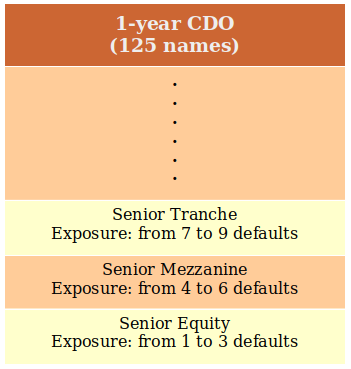
\includegraphics[width=0.5\textwidth]{figures/ex_cdo_1}
	\caption{Structure of the simple Cash CDO considered in the example.}
	\label{fig:cdo_ex_1}
\end{figure}

Assume also that one year default probabilities are identical for each bond 
($Q$) and that the correlation between each pair is also identical and equal to $\rho$.
Under these assumptions we are in the position to use the Gaussian Copula Model. 

We are interested in the expected losses for each tranche as a function of the correlation $\rho$.

The probability of having $l$ defaults, conditional to the market parameter $M$ will follow a binomial distribution given by
\begin{equation}
p(l|M) = \binom{N}{l}Q_M^l (1-Q_M)^{N-l}
\label{eq:def_prob_ex_cdo_1}
\end{equation}
where $N$ is the number of bonds in the portfolio and 
\begin{equation}
Q_M^{\textrm{corr}} = \Phi\left(\cfrac{\Phi^{-1}(Q)-\sqrt{\rho}M}{\sqrt{\-\rho}}\right)
\end{equation}
where $\Phi$ is the standard normal CDF and $Q$ the marginal probability of default 
within 1 year of a single name.

From the definition of each tranche with have that the expected losses are
\begin{itemize}
	\item $\mathbb{E}_{\textrm{equity loss}}(l, Q_M^{\textrm{corr}})=3\cdot p(l\ge 3|M) + \sum_{k=1}^{2}k\cdot p(l=k|M)$
	\item $\mathbb{E}_{\textrm{mezzanine loss}}(l, Q_M^{\textrm{corr}})=3\cdot p(l\ge 6|M) + \sum_{k=1}^{2}k\cdot p(l=k+3|M)$
	\item $\mathbb{E}_{\textrm{senior loss}}(l, Q_M^{\textrm{corr}})=3\cdot p(l\ge 9|M) + \sum_{k=1}^{2}k\cdot p(l=k+6|M)$
\end{itemize}
	
Each probability can be calculated by integrating the above with respect to $M$
	
\begin{equation} 
\mathbb{E}_{\mathrm{tranche}} = \int_{-\infty}^{\infty}{\mathbb{E}_{\mathrm{tranche}}(l, Q_M) f_M(m)dm}
\end{equation}

Let's see the corresponding \texttt{python} implementation:
first we import the necessary modules and define the needed constants.

\begin{codebox}
\begin{Verbatim}[commandchars=\\\{\}]
\PY{k+kn}{from} \PY{n+nn}{scipy}\PY{n+nn}{.}\PY{n+nn}{stats} \PY{k}{import} \PY{n}{binom}\PY{p}{,} \PY{n}{norm}
\PY{k+kn}{from} \PY{n+nn}{scipy}\PY{n+nn}{.}\PY{n+nn}{integrate} \PY{k}{import} \PY{n}{quad}
\PY{k+kn}{import} \PY{n+nn}{numpy} \PY{k}{as} \PY{n+nn}{np}
	
\PY{n}{N} \PY{o}{=} \PY{l+m+mi}{125}
\PY{n}{C} \PY{o}{=} \PY{l+m+mi}{1}
\PY{n}{R} \PY{o}{=} \PY{l+m+mi}{0}
\PY{n}{q} \PY{o}{=} \PY{l+m+mf}{0.02}
\PY{n}{tranches} \PY{o}{=} \PY{p}{[}\PY{p}{[}\PY{l+m+mi}{1}\PY{p}{,}\PY{l+m+mi}{3}\PY{p}{]}\PY{p}{,}\PY{p}{[}\PY{l+m+mi}{4}\PY{p}{,} \PY{l+m+mi}{6}\PY{p}{]}\PY{p}{,}\PY{p}{[}\PY{l+m+mi}{7}\PY{p}{,}\PY{l+m+mi}{9}\PY{p}{]}\PY{p}{]}
\end{Verbatim}
\end{codebox}

Then we define a function \texttt{p} which implements the expected losses for each tranche according to Eq.~\ref{eq:def_prob_ex_cdo_1}.
The function depends on the parameter \texttt{M}, and takes as inputs the correlation \texttt{rho} and the tranche attach-detach limits.
	
\begin{codebox}
\begin{Verbatim}[commandchars=\\\{\}]
\PY{k}{def} \PY{n+nf}{p}\PY{p}{(}\PY{n}{M}\PY{p}{,} \PY{n}{rho}\PY{p}{,} \PY{n}{lims}\PY{p}{)}\PY{p}{:}
    \PY{n}{qM} \PY{o}{=} \PY{n}{norm}\PY{o}{.}\PY{n}{cdf}\PY{p}{(}\PY{p}{(}\PY{n}{norm}\PY{o}{.}\PY{n}{ppf}\PY{p}{(}\PY{n}{q}\PY{p}{)}\PY{o}{\PYZhy{}}\PY{n}{np}\PY{o}{.}\PY{n}{sqrt}\PY{p}{(}\PY{n}{rho}\PY{p}{)}\PY{o}{*}\PY{n}{M}\PY{p}{)}\PY{o}{/}\PY{p}{(}\PY{n}{np}\PY{o}{.}\PY{n}{sqrt}\PY{p}{(}\PY{l+m+mi}{1}\PY{o}{\PYZhy{}}\PY{n}{rho}\PY{p}{)}\PY{p}{)}\PY{p}{)}
    \PY{n}{pN} \PY{o}{=} \PY{n}{binom}\PY{p}{(}\PY{n}{N}\PY{p}{,} \PY{n}{qM}\PY{p}{)}
    \PY{n}{loss} \PY{o}{=} \PY{l+m+mi}{3}\PY{o}{*}\PY{p}{(}\PY{n}{pN}\PY{o}{.}\PY{n}{cdf}\PY{p}{(}\PY{n}{N}\PY{p}{)} \PY{o}{\PYZhy{}} \PY{n}{pN}\PY{o}{.}\PY{n}{cdf}\PY{p}{(}\PY{n}{lims}\PY{p}{[}\PY{l+m+mi}{1}\PY{p}{]}\PY{o}{\PYZhy{}}\PY{l+m+mi}{1}\PY{p}{)}\PY{p}{)}
    \PY{k}{for} \PY{n}{i} \PY{o+ow}{in} \PY{n+nb}{range}\PY{p}{(}\PY{n}{lims}\PY{p}{[}\PY{l+m+mi}{0}\PY{p}{]}\PY{p}{,} \PY{n}{lims}\PY{p}{[}\PY{l+m+mi}{1}\PY{p}{]}\PY{p}{)}\PY{p}{:}
        \PY{n}{index} \PY{o}{=} \PY{n}{i}\PY{o}{\PYZhy{}}\PY{n}{lims}\PY{p}{[}\PY{l+m+mi}{0}\PY{p}{]}\PY{l+m+mi}{+1}
        \PY{n}{loss} \PY{o}{+}\PY{o}{=} \PY{n}{index}\PY{o}{*}\PY{n}{pN}\PY{o}{.}\PY{n}{pmf}\PY{p}{(}\PY{n}{i}\PY{p}{)}  
    \PY{k}{return} \PY{n}{norm}\PY{o}{.}\PY{n}{pdf}\PY{p}{(}\PY{n}{M}\PY{p}{)}\PY{o}{*}\PY{n}{loss}
\end{Verbatim}
\end{codebox}

Finally we loop over a range of possible values for the correlation on each tranche to draw the plot of the expected losses vs correlation, shown in Fig.~\ref{fig:losses_rho}.

\begin{codebox}
\begin{Verbatim}[commandchars=\\\{\}]
\PY{n}{res} \PY{o}{=} \PY{p}{[}\PY{p}{[}\PY{p}{]}\PY{p}{,}\PY{p}{[}\PY{p}{]}\PY{p}{,}\PY{p}{[}\PY{p}{]}\PY{p}{]}
\PY{k}{for} \PY{n}{i} \PY{o+ow}{in} \PY{n+nb}{range}\PY{p}{(}\PY{n+nb}{len}\PY{p}{(}\PY{n}{tranches}\PY{p}{)}\PY{p}{)}\PY{p}{:}
    \PY{k}{for} \PY{n}{rho} \PY{o+ow}{in} \PY{n}{np}\PY{o}{.}\PY{n}{arange}\PY{p}{(}\PY{l+m+mi}{0}\PY{p}{,} \PY{l+m+mf}{1.05}\PY{p}{,} \PY{l+m+mf}{0.05}\PY{p}{)}\PY{p}{:}
        \PY{k}{if} \PY{n}{rho} \PY{o}{==} \PY{l+m+mf}{1.0}\PY{p}{:}
            \PY{n}{rho} \PY{o}{=} \PY{l+m+mf}{0.99}
    \PY{n}{v} \PY{o}{=} \PY{n}{quad}\PY{p}{(}\PY{n}{p}\PY{p}{,} \PY{o}{\PYZhy{}}\PY{n}{np}\PY{o}{.}\PY{n}{inf}\PY{p}{,} \PY{n}{np}\PY{o}{.}\PY{n}{inf}\PY{p}{,} \PY{n}{args}\PY{o}{=}\PY{p}{(}\PY{n}{rho}\PY{p}{,} \PY{n}{tranches}\PY{p}{[}\PY{n}{i}\PY{p}{]}\PY{p}{)}\PY{p}{)}
    \PY{n}{res}\PY{p}{[}\PY{n}{i}\PY{p}{]}\PY{o}{.}\PY{n}{append}\PY{p}{(}\PY{n}{v}\PY{p}{[}\PY{l+m+mi}{0}\PY{p}{]}\PY{p}{)}
\end{Verbatim}
\end{codebox}

Some considerations can be done from these results. First of all, as expected, the equity tranche is the riskier, producing the highest level of loss. 

The 
\begin{equation}
\mathbb{E}_{\textrm{equity loss}} \ge \mathbb{E}_{\textrm{mezzanine loss}} \ge \mathbb{E}_{\textrm{senior loss}}
\end{equation}
relation holds only if each tranche has the same notional exposure (in our example 3).

Then we can notice that, in the equity tranche, losses are decreasing in $\rho$. When the correlation is low, indeed, the probability to have few defaults is higher than that for many. As the correlation increases, there will be more and more "simultaneous" defaults so also other tranches will start to suffer losses. In the extreme case of correlation equal to 1 all the tranches behave the same and expected losses curves join together. 

When considering all the tranches covering the entire number of names, the last tranche (the one with detachment point of 100\%) is always increasing in $\rho$. Again this can be explained with correlated defaults. 
Also, the total expected losses on the three tranches is independent of $\rho$. This is not an accident but it is due to the fact that every default scenario is affecting a tranche so that the total loss remain constant.

\begin{figure}[htb]
	\centering
	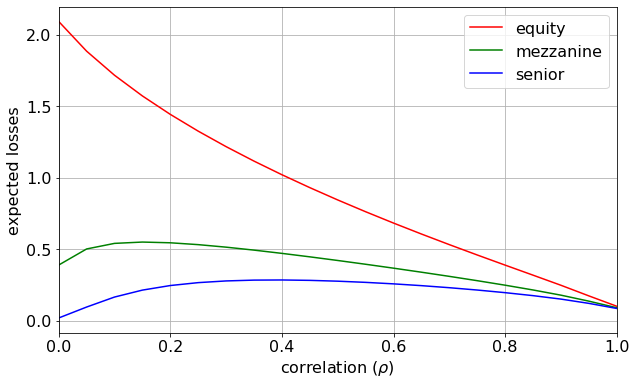
\includegraphics[width=0.7\textwidth]{figures/losses_vs_rho}
	\caption{Expected losses for each tranche as a function of the correlation parameter.}
	\label{fig:losses_rho}
\end{figure}

\begin{attention}
As noticed at the end of Section~\ref{standard-market-model}, in case the entities of the reference portfolio haven't the same default probabilities it is possible to determine Eq.~\ref{eq:def_prob_ex_cdo_1} numerically with an iterative procedure. The next snippet of code shows an example where ten names have different probabilities.

\begin{Verbatim}[commandchars=\\\{\}]
\PY{n}{N}\PY{o}{=}\PY{l+m+mi}{10}
\PY{c+c1}{\PYZsh{} probabilities of default of the each name}
\PY{n}{q} \PY{o}{=} \PY{p}{[}\PY{l+m+mf}{0.01}\PY{p}{,} \PY{l+m+mf}{0.02}\PY{p}{,} \PY{l+m+mf}{0.15}\PY{p}{,} \PY{l+m+mf}{0.22}\PY{p}{,} \PY{l+m+mf}{0.03}\PY{p}{,} \PY{l+m+mf}{0.01}\PY{p}{,} \PY{l+m+mf}{0.024}\PY{p}{,} \PY{l+m+mf}{0.008}\PY{p}{,} \PY{l+m+mf}{0.015}\PY{p}{,} \PY{l+m+mf}{0.04}\PY{p}{]}
\PY{c+c1}{\PYZsh{} p[k] probability of k defaults}
\PY{n}{p} \PY{o}{=} \PY{p}{[}\PY{l+m+mi}{0} \PY{k}{for} \PY{n}{\PYZus{}} \PY{o+ow}{in} \PY{n+nb}{range}\PY{p}{(}\PY{l+m+mi}{0}\PY{p}{,} \PY{n}{N}\PY{o}{+}\PY{l+m+mi}{1}\PY{p}{)}\PY{p}{]}
\PY{n}{p}\PY{p}{[}\PY{l+m+mi}{0}\PY{p}{]} \PY{o}{=} \PY{p}{(}\PY{l+m+mi}{1}\PY{o}{\PYZhy{}}\PY{n}{q}\PY{p}{[}\PY{l+m+mi}{0}\PY{p}{]}\PY{p}{)}
\PY{n}{p}\PY{p}{[}\PY{l+m+mi}{1}\PY{p}{]} \PY{o}{=} \PY{n}{q}\PY{p}{[}\PY{l+m+mi}{0}\PY{p}{]}

\PY{k}{for} \PY{n}{i} \PY{o+ow}{in} \PY{n+nb}{range}\PY{p}{(}\PY{l+m+mi}{2}\PY{p}{,} \PY{n}{N}\PY{o}{+}\PY{l+m+mi}{1}\PY{p}{)}\PY{p}{:}
    \PY{k}{for} \PY{n}{j} \PY{o+ow}{in} \PY{n+nb}{range}\PY{p}{(}\PY{l+m+mi}{1}\PY{p}{,} \PY{n}{i}\PY{o}{+}\PY{l+m+mi}{1}\PY{p}{)}\PY{p}{:}
        \PY{n}{p}\PY{p}{[}\PY{n}{j}\PY{p}{]} \PY{o}{=} \PY{n}{p}\PY{p}{[}\PY{n}{j}\PY{o}{\PYZhy{}}\PY{l+m+mi}{1}\PY{p}{]}\PY{o}{*}\PY{n}{q}\PY{p}{[}\PY{n}{i}\PY{o}{\PYZhy{}}\PY{l+m+mi}{1}\PY{p}{]} \PY{o}{+} \PY{n}{p}\PY{p}{[}\PY{n}{j}\PY{p}{]}\PY{o}{*}\PY{p}{(}\PY{l+m+mi}{1}\PY{o}{\PYZhy{}}\PY{n}{q}\PY{p}{[}\PY{n}{i}\PY{o}{\PYZhy{}}\PY{l+m+mi}{1}\PY{p}{]}\PY{p}{)}
    \PY{n}{p}\PY{p}{[}\PY{l+m+mi}{0}\PY{p}{]} \PY{o}{=} \PY{n}{p}\PY{p}{[}\PY{l+m+mi}{0}\PY{p}{]}\PY{o}{*}\PY{p}{(}\PY{l+m+mi}{1}\PY{o}{\PYZhy{}}\PY{n}{q}\PY{p}{[}\PY{n}{i}\PY{o}{\PYZhy{}}\PY{l+m+mi}{1}\PY{p}{]}\PY{p}{)}
		
\PY{n+nb}{print} \PY{p}{(}\PY{n}{p}\PY{p}{)}

[0.5655235318063276, 0.350403844356834, 0.11955743831716371,
0.03306691281696737, 0.007898676408014359, 0.0008119173181899153,
5.3505698491409986e-05, 2.8142380742779974e-06, 1.2554827537575903e-07,
5.2166123010999485e-09, 2.0866449204399796e-10]
\end{Verbatim}
\end{attention}

\subsection{Synthetic CDO Valuation}
Imagine a Synthetic CDO made of $N$ references in the portfolio, each one with the same notional amount (the total CDO notional is $F$).
When the $i^{th}$ reference defaults the portfolio incurs in a loss of $\frac{F}/{N}(1-R)$ (the recovery rate is assumed to be the same for all names).

The tranche loss function $TL^{L,U}(l)$ for a given time $t$ is a function of the number of defaults $l$ occurred up to that time and is given by
\begin{equation}
TL_{t}^{L,U}=\mathrm{max}(\mathrm{min}(\cfrac{l}{N}\cdot F(1-R), U)-L, 0)
\end{equation}
where $\frac{l}{N}F(1-R)$ is the total portfolio loss, if it is greater than $U$ then the tranche loss is $U$, conversely if it is lower than $L$ there is no loss.

So for example suppose $L=3\%$ and $U=7\%$ and suppose also that the portfolio loss is $5\%$. Then the tranche loss is 2\% of the total portfolio notional (or 50\% of the tranche notional $=7\%-3\%=4\%$).

When an investor \emph{sells protection} on a tranche she is guaranteeing to reimburse any realized losses on the tranche to the \emph{protection buyer} (to better understand this concept it is useful to think of the protection as an \emph{insurance}). 
In return, the protection seller receives a premium at regular intervals (typically every three months) from the protection buyer.

\subsubsection{Premium Leg}
The premium leg payments are made at the end of each time interval and are proportional to the \textbf{remaining notional} in the tranche (this is another important difference with respect to CDS, where the contract ends as soon as a default occurs).

We can then write the NPV of the premium leg as

\begin{equation}
\mathrm{NPV}_{\mathrm{premium}}^{L,U}=S\sum^{n}_{i=1}D(d_i)\cfrac{(d_i - d_{i-1})}{360}\left(F(U-L)-\mathbb{E}[TL_{d-1}^{L,U}]\right)
\label{eq:cdo_npv_premium}
\end{equation}
where $n$ is the number of payment dates, $D(d_i)$ is the discount factor, $S$ is the annualized premium. The expected value represents the notional remaining in the tranche at time $d_{i-1}$.
Note that for simplicity we are ignoring that the default may take place at any time between each payment date.

\subsubsection{Default Leg}
The default leg represents the cash flows paid to the protection buyer upon losses occurring in the considered tranche. 

The NPV of the leg can be expressed as
\begin{equation}
\mathrm{NPV}_{\mathrm{default}}^{L,U}=\sum_{i=1}^{n}D(d_i)\left(\mathbb{E}[TL_{d_i}^{L,U}]-\mathbb{E}[TL_{d_{i-1}}^{L,U}]\right)
\label{eq:cdo_npv_default}
\end{equation}
where the argument in parenthesis is the expected losses between time $d_{i-1}$ up to $d_i$. 

From Equations~\ref{eq:cdo_npv_premium} and~\ref{eq:cdo_npv_default} it is clear that the key ingredient for the valuation of a CDO is the calculation of $\mathbb{E}[TL_{d_i}^{L,U}]$ which appears in both.
Luckily using the Gaussian copula it is relatively easy to compute it. Indeed we know that 
\begin{equation}
TL_{t}^{L,U}=\mathrm{max}(\mathrm{min}(\frac{l}{N}\cdot F(1-R), U)-L, 0)
\label{eq:tl}
\end{equation}
where the only random variable is the number of defaults $l$. We also know that 
\begin{equation}
\mathbb{E}[TL_{t}^{L,U}] = \sum_{l=0}^{N}TL_{t}^{L,U}\cdot \int_{-\infty}^{\infty} DP(l(t|M)=j) \phi(M)dM
\label{eq:etl}
\end{equation}

And has we have already seen this calculation can be carried on without too much effort.
The large popularity of the Gaussian copula just resides in this, it allows to compute very quickly very complicated contracts like CDOs which usually involve a large number of correlated names.

\subsection{CDO Fair Value}
The \emph{fair value} of a CDO tranche is that value of the premium $S^*$ for which the expected value of the premium leg equals the expected value of the default leg and for what we have seen depends on the expected value of the tranche loss function.

Given Equations~\ref{eq:cdo_npv_premium} and~\ref{eq:cdo_npv_default} it can be expressed as

\begin{equation}
S^* = \cfrac{\mathrm{NPV_{default}}^{L,U}}{\sum^{n}_{i=1}D(d_i)\cfrac{(d_i - d_{i-1})}{360}\left(F(U-L)-\mathbb{E}[TL_{d-1}^{L,U}]\right)}
\label{eq:cdo_fair_value}
\end{equation}

Equation~\ref{eq:cdo_fair_value} defines the CDO fair value, but can also be used to calibrate the implied correlation parameter from the market.
This can be obtained by plugging into the equation the market premium value and solve for the correlation parameter $\rho$.
It must be noted though that the derivation of the implied correlation coefficient is not that easy since the assumed model is so simple that may not fit well to real data. Indeed it is most likely that there will be different implied $\rho$s for each tranche (while the model assumes the same correlation everywhere).

As a last consideration we have to notice that all equations shown previously have been derived under the assumptions of the same notional and recovery rate for each entity in the portfolio. Nonetheless their generalization to different notional and recovery rate is pretty straightforward.
 
%Each tranche has an attachment percentage and a detachment
%percentage. When the cumulative percentage loss of the portfolio reaches
%the attachment percentage, investors in the tranche start to lose their
%principal, and when the cumulative percentage loss of principal reaches
%the detachment percentage, the investors in the tranche lose all their
%principal and no further loss can occur to them.
%
%A common analogy compares the cash flow from the CDO's portfolio of securities (say mortgage payments from mortgage-backed bonds) to water flowing into cups of the investors where senior tranches were filled first and overflowing cash flowed to junior tranches, then equity tranches. If a large portion of the mortgages enter default, there is insufficient cash flow to fill all these cups and equity tranche investors face the losses first.

The following code implements \texttt{CollDebtObligation} class.

\begin{codebox}
\begin{Verbatim}[commandchars=\\\{\}]
\PY{k+kn}{from} \PY{n+nn}{finmarkets} \PY{k}{import} \PY{n}{DiscountCurve}\PY{p}{,} \PY{n}{CreditCurve}\PY{p}{,} \PY{n}{generate\PYZus{}swap\PYZus{}dates}
\PY{k+kn}{from} \PY{n+nn}{scipy}\PY{n+nn}{.}\PY{n+nn}{integrate} \PY{k}{import} \PY{n}{quad}
\PY{k+kn}{from} \PY{n+nn}{scipy}\PY{n+nn}{.}\PY{n+nn}{stats} \PY{k}{import} \PY{n}{norm}\PY{p}{,} \PY{n}{binom}
\PY{k+kn}{import} \PY{n+nn}{numpy} \PY{k}{as} \PY{n+nn}{np}
\PY{k+kn}{from} \PY{n+nn}{numpy} \PY{k}{import} \PY{n}{exp}\PY{p}{,} \PY{n}{sqrt}
\PY{k+kn}{from} \PY{n+nn}{datetime} \PY{k}{import} \PY{n}{date}
\PY{k+kn}{from} \PY{n+nn}{dateutil}\PY{n+nn}{.}\PY{n+nn}{relativedelta} \PY{k}{import} \PY{n}{relativedelta}
	
\PY{k}{class} \PY{n+nc}{CollDebtObligation}\PY{p}{:}
    \PY{k}{def} \PY{n+nf}{\PYZus{}\PYZus{}init\PYZus{}\PYZus{}}\PY{p}{(}\PY{n+nb+bp}{self}\PY{p}{,} \PY{n}{notional}\PY{p}{,} \PY{n}{names}\PY{p}{,} \PY{n}{tranches}\PY{p}{,} \PY{n}{rho}\PY{p}{,} \PY{n}{cc}\PY{p}{,}
                 \PY{n}{start\PYZus{}date}\PY{p}{,} \PY{n}{spreads}\PY{p}{,}
                 \PY{n}{maturity}\PY{p}{,} \PY{n}{tenor}\PY{o}{=}\PY{l+m+mi}{3}\PY{p}{,} \PY{n}{recovery}\PY{o}{=}\PY{l+m+mf}{0.4}\PY{p}{)}\PY{p}{:}
        \PY{n+nb+bp}{self}\PY{o}{.}\PY{n}{notional} \PY{o}{=} \PY{n}{notional}
        \PY{n+nb+bp}{self}\PY{o}{.}\PY{n}{names} \PY{o}{=} \PY{n}{names}
        \PY{n+nb+bp}{self}\PY{o}{.}\PY{n}{tranches} \PY{o}{=} \PY{n}{tranches}
        \PY{n+nb+bp}{self}\PY{o}{.}\PY{n}{payment\PYZus{}dates} \PY{o}{=} \PY{n}{generate\PYZus{}swap\PYZus{}dates}\PY{p}{(}\PY{n}{start\PYZus{}date}\PY{p}{,} \PY{n}{maturity} \PY{o}{*} \PY{l+m+mi}{12}\PY{p}{,} \PY{n}{tenor}\PY{p}{)}
        \PY{n+nb+bp}{self}\PY{o}{.}\PY{n}{spreads} \PY{o}{=} \PY{n}{spreads}
        \PY{n+nb+bp}{self}\PY{o}{.}\PY{n}{rho} \PY{o}{=} \PY{n}{rho}
        \PY{n+nb+bp}{self}\PY{o}{.}\PY{n}{recovery} \PY{o}{=} \PY{n}{recovery}
        \PY{n+nb+bp}{self}\PY{o}{.}\PY{n}{cc} \PY{o}{=} \PY{n}{cc}
	
    \PY{k}{def} \PY{n+nf}{one\PYZus{}factor\PYZus{}model}\PY{p}{(}\PY{n+nb+bp}{self}\PY{p}{,} \PY{n}{M}\PY{p}{,} \PY{n}{Q}\PY{p}{,} \PY{n}{l}\PY{p}{,} \PY{n}{L}\PY{p}{,} \PY{n}{U}\PY{p}{)}\PY{p}{:}
        \PY{n}{P} \PY{o}{=} \PY{n}{norm}\PY{o}{.}\PY{n}{cdf}\PY{p}{(}\PY{p}{(}\PY{n}{norm}\PY{o}{.}\PY{n}{ppf}\PY{p}{(}\PY{n}{Q}\PY{p}{)} \PY{o}{\PYZhy{}} \PY{n}{sqrt}\PY{p}{(}\PY{n+nb+bp}{self}\PY{o}{.}\PY{n}{rho}\PY{p}{)} \PY{o}{*} \PY{n}{M}\PY{p}{)} \PY{o}{/} \PY{p}{(}\PY{n}{sqrt}\PY{p}{(}\PY{l+m+mi}{1} \PY{o}{\PYZhy{}} \PY{n+nb+bp}{self}\PY{o}{.}\PY{n}{rho}\PY{p}{)}\PY{p}{)}\PY{p}{)}
        \PY{n}{b} \PY{o}{=} \PY{n}{binom}\PY{p}{(}\PY{n+nb+bp}{self}\PY{o}{.}\PY{n}{names}\PY{p}{,} \PY{n}{P}\PY{p}{)}
        \PY{k}{return} \PY{n}{b}\PY{o}{.}\PY{n}{pmf}\PY{p}{(}\PY{n}{l}\PY{p}{)} \PY{o}{*} \PY{n}{norm}\PY{o}{.}\PY{n}{pdf}\PY{p}{(}\PY{n}{M}\PY{p}{)} \PY{o}{*} \PY{n+nb}{max}\PY{p}{(}\PY{n+nb}{min}\PY{p}{(}\PY{n}{l}\PY{o}{/}\PY{n+nb+bp}{self}\PY{o}{.}\PY{n}{names} \PY{o}{*} 
               \PY{n+nb+bp}{self}\PY{o}{.}\PY{n}{notional} \PY{o}{*} \PY{p}{(}\PY{l+m+mi}{1} \PY{o}{\PYZhy{}} \PY{n+nb+bp}{self}\PY{o}{.}\PY{n}{recovery}\PY{p}{)}\PY{p}{,} \PY{n}{U}\PY{p}{)} \PY{o}{\PYZhy{}} \PY{n}{L}\PY{p}{,} \PY{l+m+mi}{0}\PY{p}{)}
	
    \PY{k}{def} \PY{n+nf}{expected\PYZus{}tranche\PYZus{}loss}\PY{p}{(}\PY{n+nb+bp}{self}\PY{p}{,} \PY{n}{d}\PY{p}{,} \PY{n}{L}\PY{p}{,} \PY{n}{U}\PY{p}{)}\PY{p}{:}
        \PY{n}{Q} \PY{o}{=} \PY{l+m+mi}{1} \PY{o}{\PYZhy{}} \PY{n+nb+bp}{self}\PY{o}{.}\PY{n}{cc}\PY{o}{.}\PY{n}{ndp}\PY{p}{(}\PY{n}{d}\PY{p}{)}
        \PY{n}{v} \PY{o}{=} \PY{l+m+mi}{0}
        \PY{k}{for} \PY{n}{l} \PY{o+ow}{in} \PY{n+nb}{range}\PY{p}{(}\PY{n+nb+bp}{self}\PY{o}{.}\PY{n}{names}\PY{o}{+}\PY{l+m+mi}{1}\PY{p}{)}\PY{p}{:}
            \PY{n}{i} \PY{o}{=} \PY{n}{quad}\PY{p}{(}\PY{n+nb+bp}{self}\PY{o}{.}\PY{n}{one\PYZus{}factor\PYZus{}model}\PY{p}{,} \PY{o}{\PYZhy{}}\PY{n}{np}\PY{o}{.}\PY{n}{inf}\PY{p}{,} \PY{n}{np}\PY{o}{.}\PY{n}{inf}\PY{p}{,} 
                     \PY{n}{args}\PY{o}{=}\PY{p}{(}\PY{n}{Q}\PY{p}{,} \PY{n}{l}\PY{p}{,} \PY{n}{L}\PY{p}{,} \PY{n}{U}\PY{p}{)}\PY{p}{)}\PY{p}{[}\PY{l+m+mi}{0}\PY{p}{]}
            \PY{n}{v} \PY{o}{+}\PY{o}{=} \PY{n}{i}
        \PY{k}{return} \PY{n}{v}
	
    \PY{k}{def} \PY{n+nf}{npv\PYZus{}premium}\PY{p}{(}\PY{n+nb+bp}{self}\PY{p}{,} \PY{n}{tranche}\PY{p}{,} \PY{n}{dc}\PY{p}{)}\PY{p}{:}
        \PY{n}{L} \PY{o}{=} \PY{n+nb+bp}{self}\PY{o}{.}\PY{n}{tranches}\PY{p}{[}\PY{n}{tranche}\PY{p}{]}\PY{p}{[}\PY{l+m+mi}{0}\PY{p}{]} \PY{o}{*} \PY{n+nb+bp}{self}\PY{o}{.}\PY{n}{notional}
        \PY{n}{U} \PY{o}{=} \PY{n+nb+bp}{self}\PY{o}{.}\PY{n}{tranches}\PY{p}{[}\PY{n}{tranche}\PY{p}{]}\PY{p}{[}\PY{l+m+mi}{1}\PY{p}{]} \PY{o}{*} \PY{n+nb+bp}{self}\PY{o}{.}\PY{n}{notional}
        \PY{n}{v} \PY{o}{=} \PY{l+m+mi}{0}
        \PY{k}{for} \PY{n}{i} \PY{o+ow}{in} \PY{n+nb}{range}\PY{p}{(}\PY{l+m+mi}{1}\PY{p}{,} \PY{n+nb}{len}\PY{p}{(}\PY{n+nb+bp}{self}\PY{o}{.}\PY{n}{payment\PYZus{}dates}\PY{p}{)}\PY{p}{)}\PY{p}{:}
            \PY{n}{ds} \PY{o}{=} \PY{n+nb+bp}{self}\PY{o}{.}\PY{n}{payment\PYZus{}dates}\PY{p}{[}\PY{n}{i} \PY{o}{\PYZhy{}} \PY{l+m+mi}{1}\PY{p}{]}
            \PY{n}{de} \PY{o}{=} \PY{n+nb+bp}{self}\PY{o}{.}\PY{n}{payment\PYZus{}dates}\PY{p}{[}\PY{n}{i}\PY{p}{]}
            \PY{n}{D} \PY{o}{=} \PY{n}{dc}\PY{o}{.}\PY{n}{df}\PY{p}{(}\PY{n}{de}\PY{p}{)}
            \PY{n}{ETL} \PY{o}{=} \PY{n+nb+bp}{self}\PY{o}{.}\PY{n}{expected\PYZus{}tranche\PYZus{}loss}\PY{p}{(}\PY{n}{ds}\PY{p}{,} \PY{n}{L}\PY{p}{,} \PY{n}{U}\PY{p}{)}
            \PY{n}{v} \PY{o}{+}\PY{o}{=} \PY{n}{D} \PY{o}{*} \PY{p}{(}\PY{n}{de} \PY{o}{\PYZhy{}} \PY{n}{ds}\PY{p}{)}\PY{o}{.}\PY{n}{days} \PY{o}{/} \PY{l+m+mi}{360} \PY{o}{*} \PY{n+nb}{max}\PY{p}{(}\PY{p}{(}\PY{n}{U} \PY{o}{\PYZhy{}} \PY{n}{L}\PY{p}{)} \PY{o}{\PYZhy{}} \PY{n}{ETL}\PY{p}{,} \PY{l+m+mi}{0}\PY{p}{)}
        \PY{k}{return} \PY{n}{v} \PY{o}{*} \PY{n+nb+bp}{self}\PY{o}{.}\PY{n}{spreads}\PY{p}{[}\PY{n}{tranche}\PY{p}{]}
	
    \PY{k}{def} \PY{n+nf}{npv\PYZus{}default}\PY{p}{(}\PY{n+nb+bp}{self}\PY{p}{,} \PY{n}{tranche}\PY{p}{,} \PY{n}{dc}\PY{p}{)}\PY{p}{:}
        \PY{n}{U} \PY{o}{=} \PY{n+nb+bp}{self}\PY{o}{.}\PY{n}{tranches}\PY{p}{[}\PY{n}{tranche}\PY{p}{]}\PY{p}{[}\PY{l+m+mi}{1}\PY{p}{]} \PY{o}{*} \PY{n+nb+bp}{self}\PY{o}{.}\PY{n}{notional}
        \PY{n}{L} \PY{o}{=} \PY{n+nb+bp}{self}\PY{o}{.}\PY{n}{tranches}\PY{p}{[}\PY{n}{tranche}\PY{p}{]}\PY{p}{[}\PY{l+m+mi}{0}\PY{p}{]} \PY{o}{*} \PY{n+nb+bp}{self}\PY{o}{.}\PY{n}{notional}
        \PY{n}{v} \PY{o}{=} \PY{l+m+mi}{0}
        \PY{k}{for} \PY{n}{i} \PY{o+ow}{in} \PY{n+nb}{range}\PY{p}{(}\PY{l+m+mi}{1}\PY{p}{,} \PY{n+nb}{len}\PY{p}{(}\PY{n+nb+bp}{self}\PY{o}{.}\PY{n}{payment\PYZus{}dates}\PY{p}{)}\PY{p}{)}\PY{p}{:}
            \PY{n}{ds} \PY{o}{=} \PY{n+nb+bp}{self}\PY{o}{.}\PY{n}{payment\PYZus{}dates}\PY{p}{[}\PY{n}{i} \PY{o}{\PYZhy{}} \PY{l+m+mi}{1}\PY{p}{]} 
            \PY{n}{de} \PY{o}{=} \PY{n+nb+bp}{self}\PY{o}{.}\PY{n}{payment\PYZus{}dates}\PY{p}{[}\PY{n}{i}\PY{p}{]}
            \PY{n}{ETL1} \PY{o}{=} \PY{n+nb+bp}{self}\PY{o}{.}\PY{n}{expected\PYZus{}tranche\PYZus{}loss}\PY{p}{(}\PY{n}{ds}\PY{p}{,} \PY{n}{L}\PY{p}{,} \PY{n}{U}\PY{p}{)}
            \PY{n}{ETL2} \PY{o}{=} \PY{n+nb+bp}{self}\PY{o}{.}\PY{n}{expected\PYZus{}tranche\PYZus{}loss}\PY{p}{(}\PY{n}{de}\PY{p}{,} \PY{n}{L}\PY{p}{,} \PY{n}{U}\PY{p}{)}
            \PY{n}{v} \PY{o}{+}\PY{o}{=} \PY{n}{dc}\PY{o}{.}\PY{n}{df}\PY{p}{(}\PY{n}{de}\PY{p}{)} \PY{o}{*} \PY{p}{(}\PY{n}{ETL2} \PY{o}{\PYZhy{}} \PY{n}{ETL1}\PY{p}{)}
        \PY{k}{return} \PY{n}{v}
	
    \PY{k}{def} \PY{n+nf}{npv}\PY{p}{(}\PY{n+nb+bp}{self}\PY{p}{,} \PY{n}{tranche}\PY{p}{,} \PY{n}{dc}\PY{p}{)}\PY{p}{:}
        \PY{k}{return} \PY{n+nb+bp}{self}\PY{o}{.}\PY{n}{npv\PYZus{}default}\PY{p}{(}\PY{n}{tranche}\PY{p}{,} \PY{n}{dc}\PY{p}{)} \PY{o}{\PYZhy{}} \PY{n+nb+bp}{self}\PY{o}{.}\PY{n}{npv\PYZus{}premium}\PY{p}{(}\PY{n}{tranche}\PY{p}{,} \PY{n}{dc}\PY{p}{)}
	
    \PY{k}{def} \PY{n+nf}{fair\PYZus{}value}\PY{p}{(}\PY{n+nb+bp}{self}\PY{p}{,} \PY{n}{tranche}\PY{p}{,} \PY{n}{dc}\PY{p}{)}\PY{p}{:}
        \PY{n}{num} \PY{o}{=} \PY{n+nb+bp}{self}\PY{o}{.}\PY{n}{npv\PYZus{}default}\PY{p}{(}\PY{n}{tranche}\PY{p}{,} \PY{n}{dc}\PY{p}{)}
        \PY{n}{den} \PY{o}{=} \PY{n+nb+bp}{self}\PY{o}{.}\PY{n}{npv\PYZus{}premium}\PY{p}{(}\PY{n}{tranche}\PY{p}{,} \PY{n}{dc}\PY{p}{)} \PY{o}{/} \PY{n+nb+bp}{self}\PY{o}{.}\PY{n}{spreads}\PY{p}{[}\PY{n}{tranche}\PY{p}{]}
        \PY{k}{return} \PY{n}{num} \PY{o}{/} \PY{n}{den}
\end{Verbatim}
\end{codebox}

Let's test the class with a CDO with 1 year maturity and a reference portfolio of 125 names. Each of them have the same default probabilities, defined through a credit curve (\texttt{cc}) and the correlation is set to 0.3. The risk free rate is flat at 5\%. The tenor has been chosen to 12 months mainly for performance reasons since the computation of the expected losses implies the integration in Equations~\ref{eq:tl} and \ref{eq:etl}, for each name, and for each payment date and this can be quite time consuming.
Tranches and premiums are defined as follows:
\begin{itemize}
	\item equity: [0.0, 0.03] (spread 0.15);
	\item mezzanine: [0.03, 0.06] (spread 0.07);
	\item senior: [0.06, 0.09] (spread 0.03);
	\item super-senior: [0.09, 1.0] (spread 0.01).
\end{itemize}

In the following example we are going to evaluate the fair value of each tranche of the contract.

\begin{codebox}
\begin{Verbatim}[commandchars=\\\{\}]
\PY{k+kn}{from} \PY{n+nn}{finmarkets} \PY{k}{import} \PY{n}{DiscountCurve}\PY{p}{,} \PY{n}{CreditCurve}
\PY{k+kn}{from} \PY{n+nn}{datetime} \PY{k}{import} \PY{n}{date}
\PY{k+kn}{from} \PY{n+nn}{dateutil}\PY{n+nn}{.}\PY{n+nn}{relativedelta} \PY{k}{import} \PY{n}{relativedelta}

\PY{n}{pillar\PYZus{}dates} \PY{o}{=} \PY{p}{[}\PY{p}{]}
\PY{n}{df} \PY{o}{=} \PY{p}{[}\PY{p}{]}
\PY{n}{observation\PYZus{}date} \PY{o}{=} \PY{n}{date}\PY{o}{.}\PY{n}{today}\PY{p}{(}\PY{p}{)}
		
\PY{k}{for} \PY{n}{i} \PY{o+ow}{in} \PY{n+nb}{range}\PY{p}{(}\PY{l+m+mi}{2}\PY{p}{)}\PY{p}{:}
    \PY{n}{pillar\PYZus{}dates}\PY{o}{.}\PY{n}{append}\PY{p}{(}\PY{n}{observation\PYZus{}date} \PY{o}{+} \PY{n}{relativedelta}\PY{p}{(}\PY{n}{years}\PY{o}{=}\PY{n}{i}\PY{p}{)}\PY{p}{)}
    \PY{n}{df}\PY{o}{.}\PY{n}{append}\PY{p}{(}\PY{l+m+mi}{1} \PY{o}{/} \PY{p}{(}\PY{l+m+mi}{1} \PY{o}{+} \PY{l+m+mf}{0.05}\PY{p}{)} \PY{o}{*}\PY{o}{*} \PY{n}{i}\PY{p}{)}
\PY{n}{dc} \PY{o}{=} \PY{n}{DiscountCurve}\PY{p}{(}\PY{n}{observation\PYZus{}date}\PY{p}{,} \PY{n}{pillar\PYZus{}dates}\PY{p}{,} \PY{n}{df}\PY{p}{)}
		
\PY{n}{cc} \PY{o}{=} \PY{n}{CreditCurve}\PY{p}{(}\PY{p}{[}\PY{n}{observation\PYZus{}date} \PY{o}{+} \PY{n}{relativedelta}\PY{p}{(}\PY{n}{years}\PY{o}{=}\PY{n}{i}\PY{p}{)} \PY{k}{for} \PY{n}{i} \PY{o+ow}{in} \PY{n+nb}{range}\PY{p}{(}\PY{l+m+mi}{5}\PY{p}{)}\PY{p}{]}\PY{p}{,}
                 \PY{p}{[}\PY{l+m+mi}{1}\PY{p}{,} \PY{l+m+mf}{0.99}\PY{p}{,} \PY{l+m+mf}{0.97}\PY{p}{,} \PY{l+m+mf}{0.95}\PY{p}{,} \PY{l+m+mf}{0.93}\PY{p}{]}\PY{p}{)}
		
\PY{n}{tranches} \PY{o}{=} \PY{p}{[}\PY{p}{[}\PY{l+m+mf}{0.0}\PY{p}{,} \PY{l+m+mf}{0.03}\PY{p}{]}\PY{p}{,} \PY{p}{[}\PY{l+m+mf}{0.03}\PY{p}{,} \PY{l+m+mf}{0.06}\PY{p}{]}\PY{p}{,} \PY{p}{[}\PY{l+m+mf}{0.06}\PY{p}{,} \PY{l+m+mf}{0.09}\PY{p}{]}\PY{p}{,} \PY{p}{[}\PY{l+m+mf}{0.09}\PY{p}{,} \PY{l+m+mf}{1.0}\PY{p}{]}\PY{p}{]}
\PY{n}{spreads} \PY{o}{=} \PY{p}{[}\PY{l+m+mf}{0.15}\PY{p}{,} \PY{l+m+mf}{0.07}\PY{p}{,} \PY{l+m+mf}{0.03}\PY{p}{,} \PY{l+m+mf}{0.01}\PY{p}{]}
		
\PY{n}{cdo} \PY{o}{=} \PY{n}{CollDebtObligation}\PY{p}{(}\PY{l+m+mf}{100e6}\PY{p}{,} \PY{l+m+mi}{125}\PY{p}{,} \PY{n}{tranches}\PY{p}{,} \PY{l+m+mf}{0.3}\PY{p}{,} \PY{n}{cc}\PY{p}{,}
                         \PY{n}{observation\PYZus{}date}\PY{p}{,} \PY{n}{spreads}\PY{p}{,} \PY{l+m+mi}{1}\PY{p}{,} \PY{l+m+mi}{12}\PY{p}{)}
\PY{k}{for} \PY{n}{i} \PY{o+ow}{in} \PY{n+nb}{range}\PY{p}{(}\PY{n+nb}{len}\PY{p}{(}\PY{n}{tranches}\PY{p}{)}\PY{p}{)}\PY{p}{:}
    \PY{n+nb}{print} \PY{p}{(}\PY{l+s+s2}{\PYZdq{}}\PY{l+s+s2}{Tranche }\PY{l+s+si}{\PYZob{}\PYZcb{}}\PY{l+s+s2}{ (}\PY{l+s+si}{\PYZob{}\PYZcb{}}\PY{l+s+s2}{): }\PY{l+s+si}{\PYZob{}:.5f\PYZcb{}}\PY{l+s+s2}{\PYZdq{}}\PY{o}{.}\PY{n}{format}\PY{p}{(}\PY{n}{i}\PY{p}{,} \PY{n}{tranches}\PY{p}{[}\PY{n}{i}\PY{p}{]}\PY{p}{,} 
                                            \PY{n}{cdo}\PY{o}{.}\PY{n}{fair\PYZus{}value}\PY{p}{(}\PY{n}{i}\PY{p}{,} \PY{n}{dc}\PY{p}{)}\PY{p}{)}\PY{p}{)}

Tranche 0 ([0.0, 0.03]): 0.15942
Tranche 1 ([0.03, 0.06]): 0.02505
Tranche 2 ([0.06, 0.09]): 0.00773
Tranche 3 ([0.09, 1.0]): 0.00017
\end{Verbatim}
\end{codebox}

As expected the equity tranche has the higher fair value being the riskier, while the senior tranche is the safest hence the one with lower premium.

\section{Complex Correlation Structures and the Financial
	Crisis}\label{complex-correlation-structures-and-the-financial-crisis}

In the derivation of the Gaussian Copula Model we have used the normal distribution. However, we could have used other and more complex
copulas as well. For example we might want to assume the correlation is
non-symmetric which is useful in finance when correlations become
very strong during market crashes and returns very negative.

In fact, Gaussian copulas are said to have played a key role in the 2008
financial crisis as tail-correlations were severely underestimated.
Consider a set of mortgages in a CDO (a particular kind of contract that will be introduced in the next Chapter): they are clearly correlated, since if one mortgage fails,
the likelihood that another failing is increased. In the early 2000s,
the banks only knew how to model the marginals of the default rates. Then an
(in)famous paper by Li~\cite{bib:copula_li} suggested to use Gaussian copulas to model the
correlations between those marginals. Rating agencies relied on this model so heavily, that severely underestimated the risk and gave false ratings\ldots

If you are interested in the argument read this paper~\cite{bib:copula_and_2008}
for an excellent description of Gaussian copulas and the Financial
Crisis, which argues that different copula choices would not have made a
difference but instead the assumed correlation was way too low.

\section{Exercises}
\begin{question}
Estimate the default probabilities for the next 5 years for 6 companies. The default correlation between each company is 0.4 and the cumulative probability of default during the next 1,2,3,4,5 years is 1\%, 2\%, 5\%, 8\%, 11\% respectively for each company.
When a Gaussian copula is used in order to simulate the defaults determine the 4th-to-default probabilities for each year.
\end{question}

\begin{solution}
\end{solution}

\begin{ipython}
from scipy.stats import multivariate_normal, norm
p_default = [0, 0.01, 0.02, 0.05, 0.08, 0.11]
mvnorm = multivariate_normal(mean=[0]*6,
cov = [[1, 0.4, 0.4, 0.4, 0.4, 0.4],
       [0.4, 1, 0.4, 0.4, 0.4, 0.4],
       [0.4, 0.4, 1, 0.4, 0.4, 0.4],
       [0.4, 0.4, 0.4, 1, 0.4, 0.4],
       [0.4, 0.4, 0.4, 0.4, 1, 0.4],
       [0.4, 0.4, 0.4, 0.4, 0.4, 1]])

n_to_default = 4
trials = 500000
result = [0., 0., 0., 0., 0., 0.]
x = mvnorm.rvs(size=trials)
for n in range(len(x)):
    p = sorted(norm.cdf(x[n]))
    for i in range(1, len(p_default)):
        if p_default[i-1] <= p[n_to_default-1] <= p_default[i]:
            result[i] += 1

print ("4th-to-default probabilies")
for i in range(len(p_default)):
    print ("{}: {:.4f}".format(i, result[i]/trials))

4th-to-default probabilies
0: 0.0000
1: 0.0004
2: 0.0009
3: 0.0059
4: 0.0098
5: 0.0135
\end{ipython}

\begin{question}
Consider a 3-year 5th-to-default basket of ten reference entities in the situation where the copula correlation is 0.15 and the expected recovery rate, \(R\), is \(40\%\). The term structure of interest rates is assumed to be flat at 3\%. The default probabilities for the ten entities are 1\%, 3\% and 7\% respectively.
Determine the breakeven rate and the NPV.
\end{question}

\begin{solution}	
\end{solution}

\begin{ipython}
from finmarkets_tot import DiscountCurve#, BasketDefaultSwaps
from datetime import date
from dateutil.relativedelta import relativedelta

n_cds = 10
rho = 0.15
l = 0.01
pillar_dates = []
df = []
observation_date = date.today()

for i in range(4):
    pillar_dates.append(observation_date + relativedelta(years=i))
    df.append(1/(1+0.03)**i)
    dc = DiscountCurve(observation_date, pillar_dates, df)

Q = [0.0, 0.01, 0.03, 0.07]
ndefaults = 5
basket = BasketDefaultSwaps(1, observation_date, 0.01, 3, 12, n_cds, rho)

print(basket.breakeven(pillar_dates, Q, dc, ndefaults))
print(basket.npv(pillar_dates, Q, dc, ndefaults))

0.0002528465216073568
0.11147956240052284
\end{ipython}

\begin{question}
Consider a Cash CDO with a maturity of 1 year, made of 125 bonds. Each bond pays a coupon of one unit after 1 year and it has not yet defaulted (the recovery rate $R$ is assumed 0). The CDO has three tranches: equity ([0, 3] defaults), mezzanine ([4, 6] defaults) 
and senior ([7, 125] defaults).
Draw the expected loss as a function of the correlation $\rho$ for the three tranches and show that the sum of the losses of each tranche is independent from $\rho$.
\end{question}

\begin{solution}	
To solve this question we need to implement a function that evaluate through the one-factor copula model and the binomial distribution the probability of $l$ defaults.
Then we can compute the expected losses for each tranche and for various values of the correlation parameter $\rho$, saving into a list the results for later plotting.
\end{solution}

\begin{ipython}
from scipy.stats import binom, norm
from scipy.integrate import quad
import numpy as np

N = 125
A = 1
R = 0
M = 1
q = 0.02
tranches = [[1,3],[4, 6],[7,125]]

def p(M, rho, lims):
    qM = norm.cdf((norm.ppf(q)-np.sqrt(rho)*M)/(np.sqrt(1-rho)))
    pN = binom(N, qM)
    prob = (lims[1]-lims[0]+1) * (pN.cdf(N) - pN.cdf(lims[1]-1))
    for i in range(lims[0], lims[1]):
        prob += (i-lims[0]+1)*pN.pmf(i)
    return norm.pdf(M)*prob

res = [[],[],[]]
for i in range(len(tranches)):
    for rho in np.arange(0., 1.05, 0.05):
        if rho == 1.0:
            rho = 0.99
        v = quad(p, -np.inf, np.inf, args=(rho, tranches[i]))
        res[i].append(v[0])
\end{ipython}

\begin{figure}[htbp]
	\begin{center}		
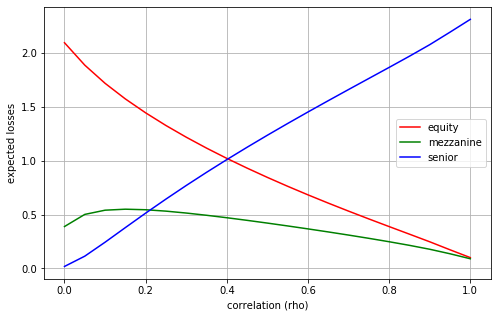
\includegraphics[width=0.7\linewidth]{figures/losses_vs_rho_2}
\end{center}
\end{figure}
To demonstrate that the total expected loss is independent from $\rho$ it is enough to print its values for a couple of different values of the correlation parameter. Since the expected loss of the tranches have been saved into lists the sum can be done among values of the lists with similar indices. 

\begin{ipython}
print (res[0][5] + res[1][5] + res[2][5])
print (res[0][10] + res[1][10] + res[2][10])
print (res[0][15] + res[1][15] + res[2][15])

2.4999999999999725
2.499999999999975
2.4999999999999774
\end{ipython}

\begin{question}
Using the \texttt{CollDebtObligation} class in the \texttt{finmarkets} module determine the fair value of each tranche in a CDO with 1 year maturity and a reference portfolio of 125 names. Each of them have the same default probabilities, 1\% and the correlation is set to 0.2. The tenor of the premium leg is 12 months. The risk free rate is flat at 5\%.
\begin{itemize}
	\item equity: [0.0, 0.03] (spread 0.20);
	\item mezzanine: [0.03, 0.06] (spread 0.01);
	\item senior: [0.06, 1.0] (spread 0.005).
\end{itemize}
How does these results change if the default probability raises to 5\% ? \\
How does these results change if instead there is an higher correlation (0.6) ?
\end{question}

\begin{solution}
\end{solution}

\begin{ipython}
from finmarkets import DiscountCurve, CreditCurve, CollDebtObligation
from datetime import date
from dateutil.relativedelta import relativedelta

pillar_dates = []
df = []
observation_date = date.today()

for i in range(2):
    pillar_dates.append(observation_date + relativedelta(years=i))
    df.append(1 / (1 + 0.05) ** i)
    dc = DiscountCurve(observation_date, pillar_dates, df)
cc = CreditCurve([observation_date + relativedelta(years=i) for i in range(5)],
    [1, 0.99, 0.97, 0.95, 0.93])
tranches = [[0.0, 0.03], [0.03, 0.06], [0.06, 0.09], [0.09, 1.0]]
spreads = [0.15, 0.07, 0.03, 0.01]
cdo = CollDebtObligation(100e6, 125, tranches, 0.3, cc,
    observation_date, spreads, 1, 12)
for i in range(len(tranches)):
    print ("Tranche {} ({}): {:.5f}".format(i, tranches[i], cdo.fair_value(i, dc)))

Tranche 0 ([0.0, 0.03]): 0.17775
Tranche 1 ([0.03, 0.06]): 0.01570
Tranche 2 ([0.06, 1.0]): 0.00012
\end{ipython}
With an higher default probability instead, the NPV of the default leg increases and so does the fair value.

\begin{ipython}
Tranche 0 ([0.0, 0.03]): 0.59296
Tranche 1 ([0.03, 0.06]): 0.22714
Tranche 2 ([0.06, 1.0]): 0.00530
\end{ipython}
Finally with a larger correlation the probability of multiple defaults increases leading to larger losses in safer tranches. So the fair value increases in mezzanine and senior tranches, but is lower in the equity where the probability of few defaults is reduced.

\begin{ipython}
Tranche 0 ([0.0, 0.03]): 0.09899
Tranche 1 ([0.03, 0.06]): 0.03498
Tranche 2 ([0.06, 1.0]): 0.00192
\end{ipython}


\begin{thebibliography}{9}
\bibitem{bib:cdo} J. C. Hull, \emph{Options, Futures and Other Derivatives, 7th Ed.}, Credit Derivatives (Ch. 23), Pearson Prentice Hall, 2009
\bibitem{bib:copula_and_2008} S. Watts, \href{http://samueldwatts.com/wp-content/uploads/2016/08/Watts-Gaussian-Copula_Financial_Crisis.pdf}{\emph{Gaussian Copula and Financial Crisis}} [Online]
\bibitem{bib:copula_li}D. X. Li, \href{http://www.maths.lth.se/matstat/kurser/fmsn15masm23/default.pdf}{\emph{On Default Correlation: A Copula Function Approach}}, RiskMetrics Group, 2000 [Online]
\end{thebibliography}
